\chapter{Gerenciamento do Sistema de Filtragem}
\label{chap:pm}

O sistema de filtragem de alto nível do ATLAS é um ambiente em constante evolução. Diariamente, milhares de colaboradores deste ambiente apresentam melhorias, como, por exemplo, parâmetros mais eficientes para a calibração dos detetores,  simulações de Monte Carlo mais fidedignas, ou atualizações do \emph{software} desenvolvido para o sistema de filtragem. Adicionalmente, novas técnicas de processamento de sinais precisam ser validada neste ambiente, para que possam ser incorporadas com segurança ao sistema de filtragem e utilizadas durante a operação nominal do LHC. A complexidade do sistema de filtragem do ATLAS exige um grande tempo de aprendizado para que um colaborador esteja minimamente familiarizado, de forma que possa validar novas técnicas de filtragem \emph{online} neste ambiente. Adicionalmente, a necessidade constante de testes deste ambiente resultam na necessidade de mecanismos de automação que permitam a configuração e a execução do sistema de filtragem, de forma que desenvolvedores de técnicas de filtragem \emph{online} possam dedicar-se somente a seus estudos, abstraindo-se da complexidade de gerenciamento deste sistema. Adicionalmente, a automatização permite que mecanismos de validação automáticos sejam desenvolvidos, permitindo que melhorias do sistema de filtragem possam ser testadas sob diversas condições de operação em um espaço de tempo consideravelmente reduzido.

Este capítulo apresenta os mecanismos de gerenciamento automatizado desenvolvidos para permitir que as pesquisas de processamento de sinais abordadas neste trabalho pudessem ser validadas junto ao sistema de filtragem de alto nível do ATLAS, para serem incorporadas oficialmente por este ambiente. Inicialmente, os mecanismos desenvolvidos estavam destinados a gerir apenas o segundo nível de filtragem, visto ser este o local onde as análises desenvolvidas serão implementadas. Entretanto, os projetos desenvolvidos provaram-se de tal forma versáteis, que, no âmbito da colaboração com o projeto ATLAS, foram rapidamente expandidos de forma a abranger todo o sistema de filtragem de alto nível, resultando em grandes ganhos para a colaboração. 

Este capítulo apresenta a seguinte organização: a sessão~\ref{sec:oks} apresentará o serviço de base de dados de configuração existente no sistema de filtragem de alto nível, e que fornece, a todos os aplicativos do sistema de filtragem, seus parâmetros de configuração. Em seguida, a sessão~\ref{sec:pm} apresentará o primeiro mecanismo de automação desenvolvido, que destina-se a criar os parâmetros de configuração necessários para operar o \emph{trigger}. Por fim, a sessão\ref{sec:runner} apresentará o ambiente para execução automática do sistema de filtragem do ATLAS.


\section{O Servidor de Base de Dados}
\label{sec:oks}

Conforme visto no capítulo~\ref{chap:sistema_filtragem}, a parte de alto nível do sistema de filtragem (composto pelos LVL2 e EF) é composta por milhares de aplicativos, desenvolvidos em linguagem de programação de alto nível, executados em computadores de uso geral com sistemas operacionais do tipo UNIX, conectados por redes \emph{ethernet} de alta velocidade. Isto proporciona enorme ganho no que tange a capacidade de configuração do sistema de filtragem de alto nível. É permitido configurar parâmetros como quais módulos do sistema de filtragem estarão disponíveis, quando e em que nó uma dada aplicação deve ser inicializada, como monitorar processos em execução e como proceder em caso de erros, etc. Consequentemente, antes de iniciar a operação do sistema de filtragem de alto nível do ATLAS, cada grupo responsável por uma determinada parte do sistema de filtragem deve fornecer os parâmetros de configuração da mesma. Durante a inicialização do sistema de filtragem, estes parâmetros de configuração serão acessados por milhares de processos simultaneamente. Adicionalmente, qualquer mudança feita em um dado parâmetro de configuração deve ser notificada a todos os processos em execução para que os processos impactados por tal mudança seja reconfigurados de acordo. Por fim, as configurações utilizadas precisam ser arquivadas para referências futuras por parte dos colaboradores do sistema de filtragem do ATLAS. Estes requisitos  tornam as aplicações de base de dados comercialmente existentes inviáveis, resultando na necessidade de criar-se uma base de dados própria, capaz de atender a estes requisitos. 

Com esta finalidade, foi desenvolvido a base de dados OKS (\emph{Object Kernel Support}) \cite{bib:oks}. No OKS, cada aplicação ou recurso do sistema de filtragem é descrito como uma classe em uma base de dados de \emph{schema}. Esta base contém a descrição de todas as classes, os atributos disponíveis, relações de herança e dependência com outras classes, etc, de acordo com o conceito de programação orientada a objetos \cite{bib:poo}. Adicionalmente, o OKS fornece um ambiente onde o usuário pode descrever como gostaria de configurar o sistema de filtragem de alto nível, através do instanciamento e configuração de parâmetros das classes contidas no \emph{schema} e, ao final, gerar uma base de dados de configuração. Esta base será, no momento da inicialização do sistema de \emph{trigger}, lida por um aplicativo de controle, que será responsável por inicializar cada um dos aplicativos do sistema de filtragem em seus respectivos nós de processamento. Em seguida, cada aplicação deverá acessar esta base de dados de configuração de forma a configurar parâmetros que digam respeito ao seu funcionamento em especial (tamanho de filas, protocolo de comunicação a ser usado, valores de \emph{timeout}, etc).  

\begin{figure}
\begin{center}
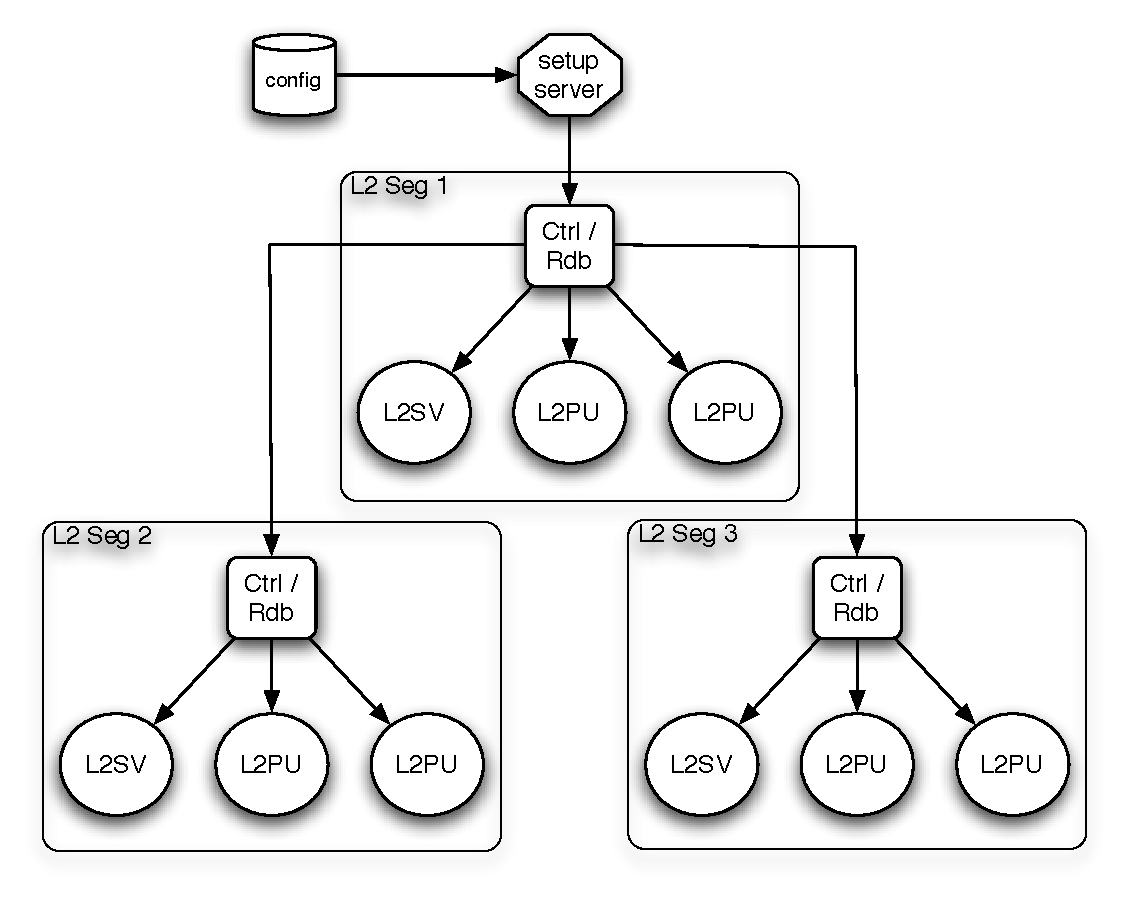
\includegraphics[width=0.6\textwidth]{oks_multi_control_strategy}
\caption{Estrutura de controle hierárquico do sistema de filtragem.}
\label{fig:multi_control}
\end{center}
\end{figure}

Para garantir sua escalabilidade, o sistema de filtragem pode ser dividido, logicamente, em \emph{segmentos}. Cada segmento contém sempre um controlador responsável por gerir os aplicativos dentro daquele segmento. Adicionalmente, utilizam-se múltiplos servidores de configuração, para evitar gargalos durante a fase de configuração. É apresentado, na Fig.~\ref{fig:multi_control}, um exemplo desta abordagem de controle hierárquico através da utilização de múltiplos segmentos. Como se percebe, ao multiplicar-se o número de aplicações de controle, diminui-se a carga de operações em cada controlador, permitindo que o número de aplicações aumente indefinidamente.  

Para a geração da base de dados de configuração, bem como a leitura da mesma, o ambiente OKS oferece interfaces de acesso em C++. Desta forma, o usuário fica isento dos detalhes de implementação e de localização da base de dados (local ou remota). Entretanto, a tarefa de configurar cada objeto, bem como a relação entre eles e sua organização lógica em segmentos, ainda fica a cargo do usuário, o que representa uma tarefa bastante penosa e delicada, requerendo conhecimento especialista, nem sempre disponível.


\section{O \emph{PartitionMaker}}
\label{sec:pm}

No início do desenvolvimento do sistema de filtragem de alto nível, as partições de configuração eram criadas manualmente, visto que a partição é um arquivo texto contendo os objetos descritos em linguagem XML \cite{bib:xml}. Entretanto, esta solução tornou-se rapidamente inviável devido ao grande número de componentes a serem configurados.

A primeira abordagem automática para a criação de base de dados de configuração era baseada em \emph{templates}. Nesta abordagem, o código XML de um objeto de cada classe ficava descrito como um modelo em um arquivo texto. Apenas alguns parâmetros podiam ser configurados, e os demais tinham valores pré-fixados. O usuário era, então, obrigado a configurar todos os parâmetros variáveis, o que restringia a utilização da ferramenta apenas aos usuários experientes. A falta de testes de consistência dos valores configurados resultava em freqüentes execuções mal sucedidas do sistema de filtragem. Por fim, como a descrição de cada objeto estava fixada, qualquer mudança na classe de um dado objeto, ou na implementação da base de dados, inutilizava a ferramenta de configuração até que o desenvolvedor da mesma atualizasse a sua base de \emph{templates}.

\begin{figure}
\begin{center}
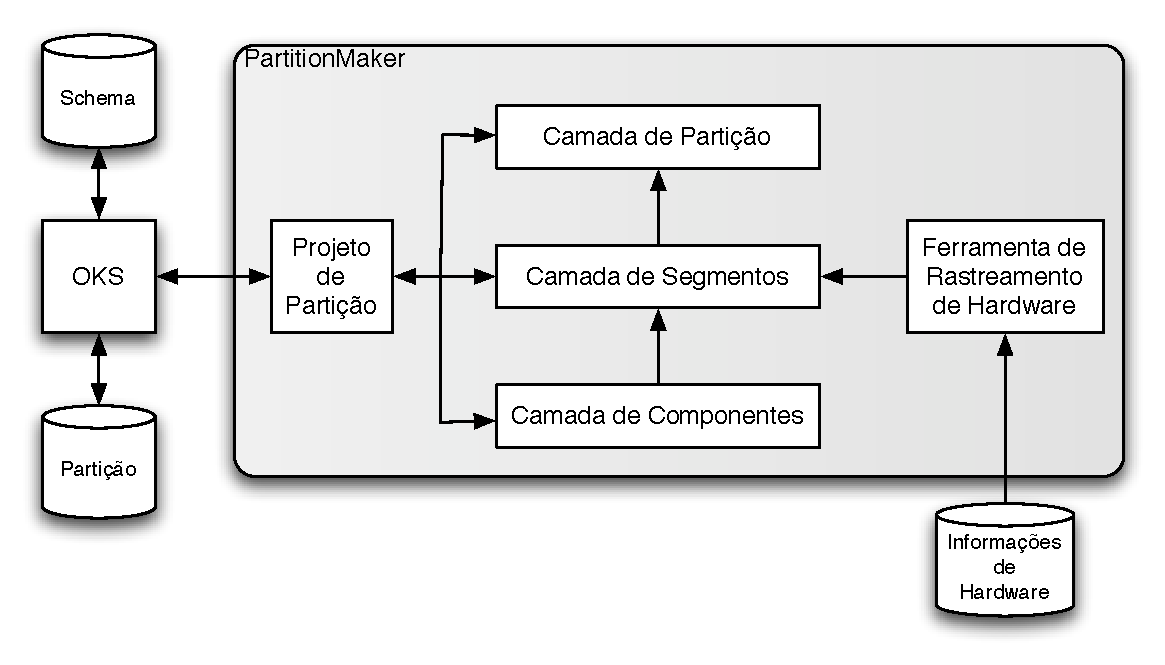
\includegraphics[width=0.65\textwidth]{partitionmaker_block_diagram}
\caption{Diagrama em blocos do \emph{PartitionMaker}.}
\label{fig:pm}
\end{center}
\end{figure}

Para se obter configuração automatizada, superando as falhas observadas nas abordagens anteriores, o \emph{PartitionMaker}, cujo diagrama é apresentado na Fig.~\ref{fig:pm}, foi desenvolvido. A filosofia deste ambiente é agregar o conhecimento especialista a respeito do sistema de filtragem, de forma que os usuários com diferentes níveis de conhecimento sobre o sistema de filtragem possam ser conduzidos com segurança durante o processo de configuração, resultando em execuções otimizadas e minimizando as possibilidades de erros. Por fim, o ambiente deve operar integrado à base de dados OKS, de forma a garantir que mudanças ocorridas na classe de um dado objeto sejam imediatamente reconhecidas pelo \emph{PartitionMaker}.

Ao ser inicializado pelo usuário, o \emph{PartitionMaker} lê a base de dados de \emph{schema} e gera uma representação em \emph{Python} \cite{bib:python} de cada uma das classes existentes. Esta leitura é realizada utilizando \emph{bindings} de C++ para Python \cite{bib:boost}, permitindo que o \emph{PartitionMaker} usufrua dos recursos já implementados na base de dados OKS, além de isentar o \emph{PartitionMaker} dos detalhes de implementação da base de dados de configuração e \emph{schema}. Toda esta operação de comunicação com o OKS é realizada pelo módulo de  \emph{Projeto de Partição}, de forma a abstrair do resto do sistema os detalhes desta comunicação.

\begin{figure}[t]
\begin{center}
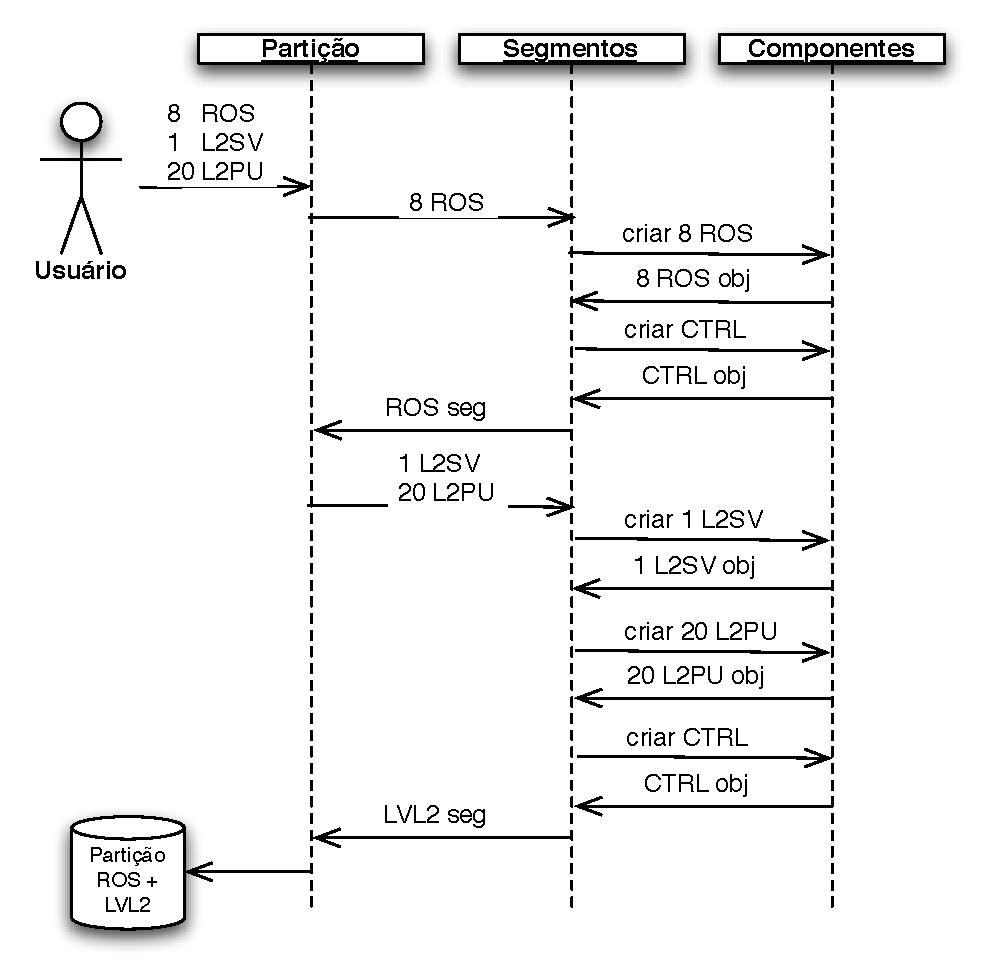
\includegraphics[width=0.6\textwidth]{partitionmaker_generation_flow}
\caption{Exemplo de fluxo de geração de uma partição.}
\label{fig:pm_flow}
\end{center}
\end{figure}

Após a inicialização, o usuário recorre aos diversos módulos e funções disponíveis, para atingir seus objetivos de configuração. De forma a atender uma vasta gama de usuários, com diferentes graus de familiaridade com o sistema de filtragem, uma abordagem em três camadas foi utilizada.

A camada mais baixa (\emph{Camada de Componentes}) é responsável por configurar cada objeto OKS individualmente. O controle de consistência, nesta camada, restringe-se a verificar se os limites aceitáveis para determinados atributos, tipo de dado inserido, entre outros, fazem sentido. Os objetos OKS são criados utilizando-se as funções da  base de dados OKS, evitando a replicação de código.

A segunda camada (\emph{Camada de Segmentos}) responsabiliza-se por acessar os objetos configurados pela primeira e agrupá-los na forma de segmentos com significado lógico para o sistema de filtragem. É de responsabilidade desta camada assegurar que as relações entre as aplicações dentro de um mesmo segmento estejam corretas, e que as aplicações contidas no mesmo apresentam relações entre si (por exemplo, evitando que uma aplicação do filtro de eventos esteja presente em um segmento destinado ao segundo nível). 

A última camada (\emph{Camada de Partição}) se encarrega de agrupar os segmentos gerados em uma base final de configuração, chamada de \emph{partição}, podendo esta ser finalmente utilizada para executar o sistema de filtragem. Nesta camada, é verificada se a relação entre segmentos está correta, para que os mesmos operem em harmonia.

Com esta abordagem multi-camada, usuários mais inexperientes com o ambiente e o sistema de filtragem podem trabalhar apenas na camada superior, de forma que, ao fornecerem poucos parâmetros gerais (número de processadores a serem utilizados, quais níveis devem ser executados, etc), o \emph{PartitionMaker} fornecerá uma base de configurações otimizada para os objetivos do usuário. Valores mais específicos são automaticamente calculados, graças ao conhecimento especialista agregado. Já usuários mais experientes, para atenderem casos de uso mais específicos, podem recorrer às camadas mais baixas do sistema. Usuários podem, inclusive, combinar recursos de várias camadas, por exemplo, gerando uma configuração padrão com a camada mais alta, e com recursos da camada mais baixa, alterar seus objetos e segmentos de acordo com suas necessidades especiais.

\begin{figure}[t]
\begin{center}
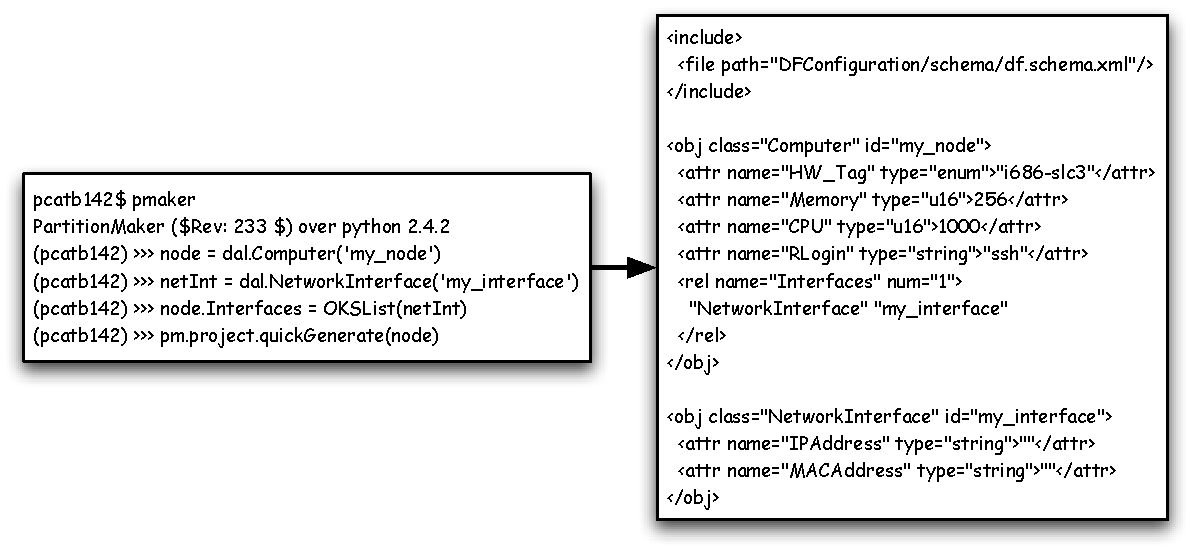
\includegraphics[width=0.7\textwidth]{ide}
\caption{Exemplo de geração de uma partição.}
\label{fig:ide}4
\end{center}
\end{figure}

É apresentado na Fig.~\ref{fig:pm_flow} um exemplo simplificado do fluxo de mensagens para a criação de uma partição contendo 8 ROS, além do LVL2 contendo 1 L2SV e 20 L2PU. No exemplo, o usuário trabalha somente com a camada mais alta. Ao especificar somente o número de componentes desejados, a camada de partição dispara mensagens para a camada de segmentos, de forma que sejam criados os segmentos para os ROS e LVL2. A camada de segmentos, por sua vez, ativa a camada de componentes, de forma que cada um dos objetos necessários sejam criados e retornados à camada de segmentos. Em seguida, a camada de segmentos agrupa tais componentes de maneira coerente à sua função, e os segmentos gerados são retornados para a camada de partição, para que sejam conectados e finalmente retornados ao usuário.

Outra etapa importante no processo de configuração é selecionar os nós de processamento a serem utilizados por cada aplicação. Para tal, o Módulo de Rastreamento de \emph{Hardware} permite rastrear um conjunto de máquinas de forma a analisar a propriedade destas (velocidade de \emph{clock}, quantidade de memória, interfaces de rede, etc), para melhor definir quais aplicações devem rodar em quais máquinas. Esta busca é feita em paralelo, através da utilização de várias \emph{threads} \cite{bib:modern_operating_systems} de execução, usando a estrutura de rede disponível. Isto resulta em tempos de busca bastante reduzidos, na ordem de poucas dezenas de segundos, para um conjunto de várias centenas de máquinas. 

Ao final deste processo de configuração, obtém-se uma representação da base de dados de configuração através de objetos em \emph{Python}. Esta base é então exportada, utilizando-se os recursos do módulo \emph{Projeto de Partição}, para o formato OKS de base de dados de configuração, podendo, finalmente, ser utilizada para a operação do sistema de filtragem de alto nível do ATLAS. Este módulo também permite que bases de dados de configuração já criadas possam ser importadas e editadas dentro do \emph{PartitionMaker}, proporcionando, desta maneira, que partições geradas com recursos externos ao \emph{PartitionMaker} também possam ser manipuladas neste ambiente.

Por ser implementado em \emph{Python}, o \emph{PartitionMaker} pode usufruir dos recursos bastante numerosos  desta linguagem. Como conseqüência, um ambiente integrado de desenvolvimento está disponível, permitindo rápida prototipagem de base de dados de configuração, conforme o exemplo na Fig.~\ref{fig:ide} demonstra. Ao inicializar o ambiente integrado, através do comando \texttt{pmaker}, o usuário acessa as funcionalidades do sistema. No exemplo, deseja-se configurar um nó de execução (\texttt{my\_node}) contendo uma interface de rede (\texttt{my\_interface}), usando, neste caso, a \emph{Camada de Componentes}. Ao final da configuração, os objetos criados em \emph{Python} são exportados para o formato utilizado pelo OKS através da função \texttt{quickGenerate}, cujo resultado aparece ao lado direito da Fig.~\ref{fig:ide}.

A facilidade da linguagem \emph{Python}, aliada ao ambiente integrado de desenvolvimento, permite que \emph{plugins} possam ser facilmente desenvolvidos para o \emph{PartitionMaker},  expandindo consideravelmente a capacidade do trabalho proposto. Por fim, como o ambiente integrado aceita comandos, tanto manualmente inseridos, bem como oriundos de um arquivo texto, \emph{scripts} de configuração podem ser escritos com facilidade, permitindo a execução de testes automáticos do sistema de filtragem do ATLAS, quando se deseja observar o comportamento deste sob diversas condições de operação (número de processadores, níveis de filtragem considerados, etc).

A abordagem utilizada para a concepção do \emph{PartitionMaker} resultou num claro aumento da produtividade dos desenvolvedores e operadores do sistema de filtragem do ATLAS. Antes, era necessária a presença de especialistas para garantir a correta configuração do sistema de filtragem. Com este conhecimento especialista embutido no \emph{PartitionMaker}, os usuários ficam mais independentes durante o processo de configuração. Isto resulta, também, em ganhos de produtividade para os técnicos especialistas, visto que minimiza-se a necessidade destes interromperem suas atividades para apoiar usuários menos experientes.

Outro resultado obtido foi a considerável diminuição de execuções mal sucedidas para os testes do sistema de filtragem do ATLAS. Com o \emph{PartitionMaker} identificando e notificando automaticamente possíveis erros durante a configuração, possíveis falhas podem ser identificadas antes da execução do sistema de filtragem, evitando-se a interrupção da operação do experimento.


\section{Execução Automática do Sistema de Filtragem}
\label{sec:runner}

Embora o processo de configuração possa ser totalmente automatizado, sua execução ainda é um processo manual, requerendo os seguintes passos:

\begin{enumerate}

\item \textbf{Inicialização}: neste ponto, a base de configuração é lida, e os aplicativos de controle posicionados no nível mais alto são inicializados. Em seguida, todos os aplicativos ligados a este controlador são inicializados, bem como todos os controle do nível imediatamente abaixo. Por sua vez, este controles inicializam suas aplicações, numa reação em cadeia, até que todo o sistema de filtragem esteja ativado. Neste ponto, todos os servidores RDB também se encontram ativos, para proverem os parâmetros de configuração na etapa seguinte.

\item \textbf{Configuração}: durante esta fase, os parâmetros de configuração são lidos da base de dados pelo controlador de mais alto nível, e são propagados pelos servidores RDB pelo resto da infra-estrutura, para evitar gargalos de acesso à base de dados de configuração. Em seguida, cada aplicativo acessa seus parâmetros de configuração, ficando, ao final, prontos para o início da operação do sistema de filtragem.

\item \textbf{Execução}: nesta etapa, o sistema de filtragem acessa os eventos que interagiram com os detetores do ATLAS, ou os arquivos de simulação de Monte Carlo passados (em caso de simulação) e realiza a filtragem propriamente dita. Durante a execução, informações de operação de toda a infra-estrutura são amostradas e utilizadas para a produção de histogramas e gráficos \emph{online}, para serem analisados pelos operadores do sistema de filtragem, ou por mecanismos de monitoração automáticos. Nesta etapa arquivos de \emph{log} também são produzidos, por cada aplicação, para serem analisados pelos desenvolvedores em caso de falhas de execução de um determinado módulo. Este estado é mantido até que a ordem de interrupção do sistema de filtragem seja fornecida pelos operadores.

\end{enumerate}

Embora ativar manualmente cada um dos passos descritos acima seja razoável durante a operação nominal do experimento, esta tarefa tende a ser bastante tediosa quando é necessário executar o sistema de filtragem muitas vezes, como é o caso de testes de validação de novas versões do TDAQ e de novos \emph{hardwares} incorporados ao projeto. Adicionalmente, a ativação manual do sistema de filtragem impossibilita que testes automáticos sejam realizados. 

\begin{figure}
\begin{center}
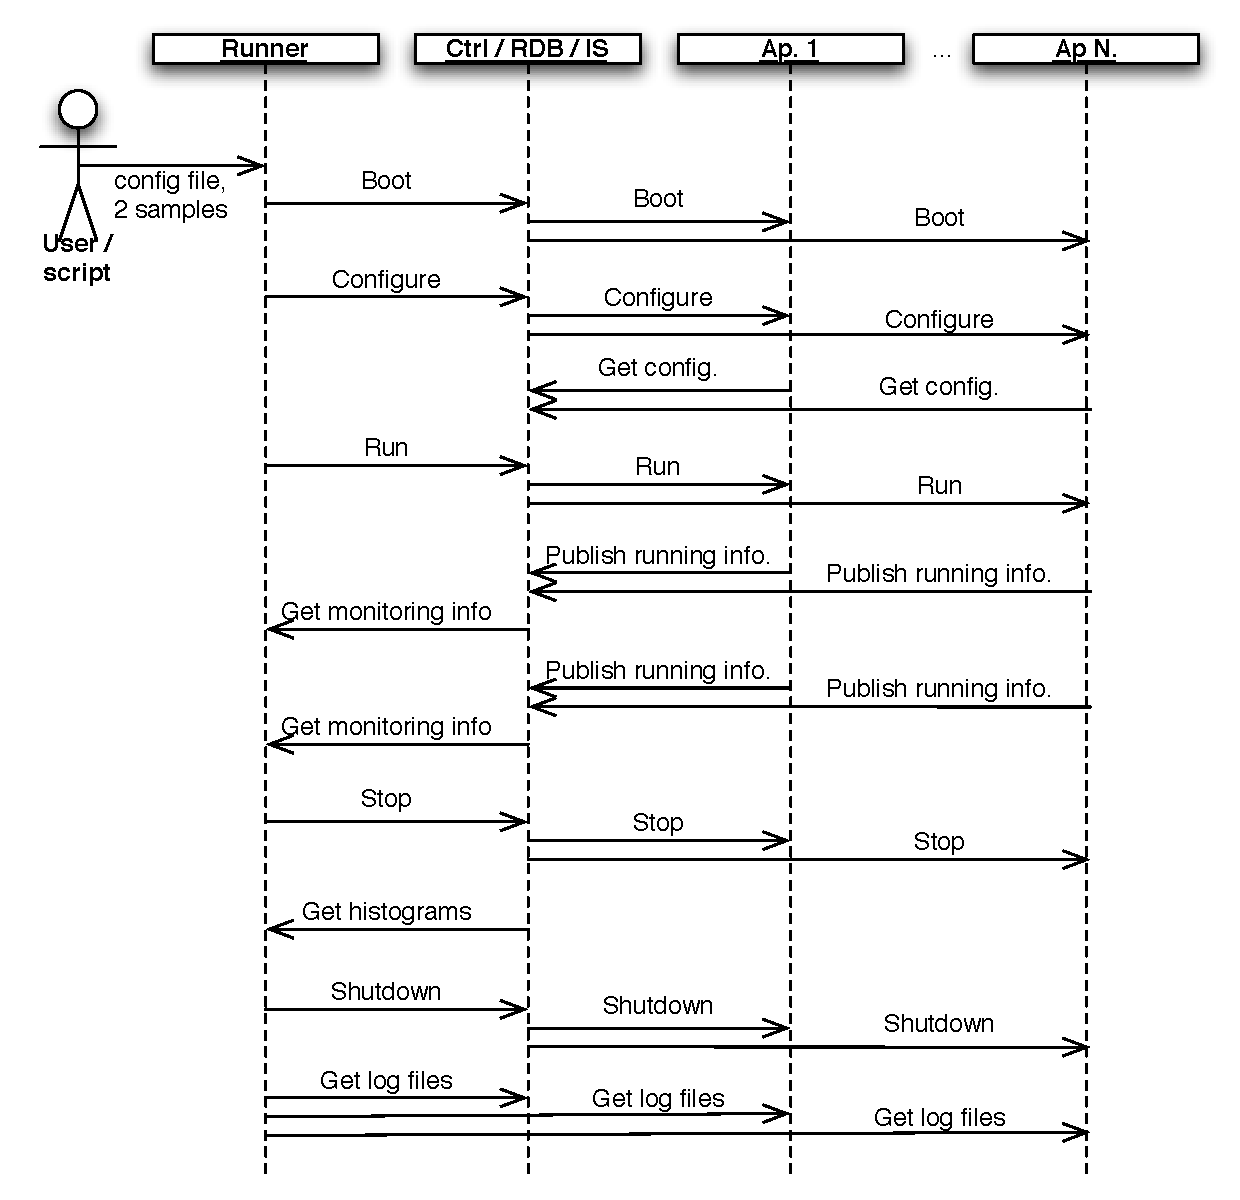
\includegraphics[width=0.6\textwidth]{runner_execution_flow}
\end{center}
\caption{Runner execution flow example.}
\label{fig:runner_exec_flow}
\end{figure}

Para suprir esta necessidade de execução automatizada do sistema de filtragem, o \emph{Runner} foi desenvolvido. Seu principal objetivo é prover uma maneira automatizada de executar o TDAQ, gerindo automaticamente todas as suas etapas de execução, e recolhendo automaticamente as informações de monitoração e \emph{logs} de execução, provendo ao final, se desejado, um relatório final de execução. É apresentado na figura~\ref{fig:runner_exec_flow} um exemplo generalizado do fluxo de comandos do \emph{Runner}. Neste exemplo, o usuário (um \emph{script} de execução, por exemplo) provê a base de dados de configuração e requisita ao \emph{Runner} que o TDAQ seja executado por tempo suficiente para que duas amostras de informações de monitoração possam ser adquiridas. Primeiramente, o \emph{Runner} envia a mensagem para o controlador de mais alto nível do TDAQ para que o mesmo inicialize a infra-estrutura do sistema de filtragem. Este controlador, por sua vez, propaga a mensagem para a inicialização. Em seguida, de maneira análoga, o comando para a configuração do TDAQ é propagado, e, cada módulo acessa seus parâmetros de configuração do servidor RDB a que está conectado. Na seqüência, o sistema de filtragem é inicializado, e cada aplicativo publica suas informações de monitoração no servidor IS ao qual está conectado, e este produz, também, os histogramas \emph{online} com a estatística obtida com a execução do TDAQ. Em paralelo, o \emph{Runner} acessa este servidor de IS para recolher as informações já publicadas. Após a aquisição de duas amostras de monitoração, o \emph{Runner} envia a instrução para a interrupção da execução do sistema de filtragem, sendo esta propagada por todo o TDAQ. Após a interrupção, os histogramas gerados são copiados de cada servidor IS para a máquina onde o \emph{Runner} está sendo executado. Em seguida, o \emph{Runner} ordena a finalização de todos os aplicativos, e, após o término dos mesmos, conecta remotamente a cada um dos nós utilizados para a execução do TDAQ, recolhendo os arquivos de \emph{log} gerados durante o processo. Ao final, as variáveis de monitoração, histogramas \emph{online} e \emph{logs} de execução estão todos concentrados na máquina do usuário, e disponíveis para análise \emph{offline}.

O \emph{Runner} apresenta-se como um conjunto de módulos em \emph{Python}. Desta forma, a mesma IDE e linguagem de sintaxe disponível para o \emph{PartitionMaker} estão disponível para este ambiente. Consequentemente, \emph{plugins} e \emph{scripts} de configuração podem ser facilmente desenvolvidos para este ambiente.

Ao combinar-se os recursos do \emph{Runner} com o \emph{PartitionMaker}, aliados com ferramentas de análise com interface em \emph{Python}, como o \emph{ROOT} \cite{bib:root}, obtém-se automatização total de todo o processo necessário para a execução do sistema de filtragem do ATLAS, aumentando consideravelmente a capacidade de produzir mecanismos de validação eficientes, fazendo com que os desenvolvedores do TDAQ possam se abstrair de detalhes do processo de execução do TDAQ, ficando sua atenção exclusivamente no desenvolvimento de módulos de sua competência. 
